\section{Задача № 3}

Дано тело Т, ограниченное следующими поверхностями: $y+\sqrt{x^2+z^2}=0, x^2+z^2=1, x^2+y+z^2=2$.

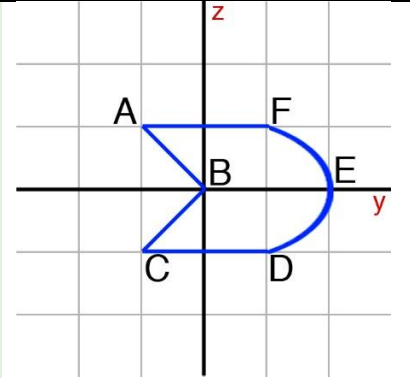
\includegraphics[scale=0.5]{images/Input_task3.png}

\begin{enumerate}
    \item Изобразите тело Т на графике в пространстве.
    \item Вычислите поток поля $\Vec{a} = ( \sin{zy^2})\Vec{i} + \sqrt{2}x\Vec{j} + (\sqrt{2+y}-3z)\Vec{k}$ через боковую поверхность тела Т, образованную вращением дуги $AFEDC$ вокруг оси $Oy$, в направлении внешней нормали поверхности тела Т.
\end{enumerate}

\subsection{Решение}
\begin{enumerate}
    \item Изобразите тело Т на графике в пространстве.
    
    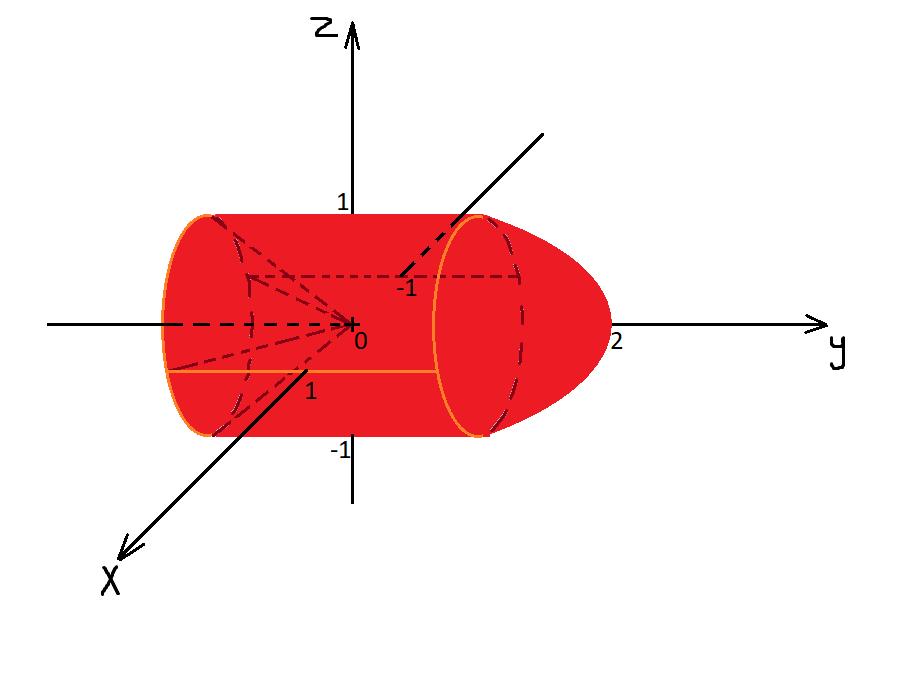
\includegraphics[scale = 0.5]{images/Math_RW4_task3.png}

    \item Вычисление потока

    Поток векторного поля через поверхность - это поверхностный интеграл второго рода по поверхности.

    $\Pi = \iint\limits_{S} P(x,y,z)dydz + Q(x,y,z)dxdz + R(x,y,z)dxdy$

    Векторное поле определено так: 
    
    $\Vec{a} = P(x,y,z)\Vec{i} + Q(x,y,z)\Vec{j} + R(x,y,z)\Vec{k} = (\sin{zy^2})\Vec{i} + \sqrt{2}x\Vec{j} + (\sqrt{2+y}-3z)\Vec{k}$

    Тогда можно получить:
    \begin{align*}
        &P(x,y,z) = \sin{zy^2}\\ 
        &Q(x,y,z) = \sqrt{2}x\\ 
        &R(x,y,z) = \sqrt{2+y}-3z
    \end{align*}

    Поток векторного поля обладает свойством аддитивности, поэтому, чтобы найти поток через поверхность, образованную вращением дуги $AFEDC$ вокруг оси $Oy$, найдем поток через замкнутую поверхность ($AFEDC$ замкнутая кривая, вращение вокруг оси $Oy$), затем вычтем поток через поверхность, образованную вращением отрезка $AC$ вокруг оси $Oy$.

    \textbf{Теорема Гаусса-Остроградского}. Поток векторного поля $\Vec{a}$ через замкнутую кусочно-гладкую поверхность  $S$  в направлении внешней нормали равен тройному интегралу от  $div \Vec{a}$  по области  $V$, ограниченной поверхностью  $S$.
    
    Поток через замкнутую поверхность ($\Pi_{0}$) найдем по формуле Гаусса-Остроградского:
    \begin{equation*}
        \Pi_{0} = \iiint_{V}div\Vec{a}\; dV
    \end{equation*}

    Вычислим дивергенцию поля:
    \begin{equation*}
        div\Vec{a} = \frac{\partial P(x,y,z)}{\partial x} + \frac{\partial Q(x,y,z)}{\partial y} + \frac{\partial R(x,y,z)}{\partial z} = 0 + 0 - 3 = -3
    \end{equation*}
    
    Порядок обхода тела:
    \begin{align*}
        -1 \leq &x \leq 1 \\
        -\sqrt{1-x^2} \leq &z \leq \sqrt{1-x^2} \\
        -1 \leq &y \leq 2 - x^2 - z^2
    \end{align*}

    Вычисление:
    \begin{align*}
        \Pi_{0} = \iiint_{V}div\Vec{a}\; dV = \iiint_{V}-3\; dV = -3\iiint_{V}dV =\\= 
        -3\int_{-1}^{1}dx\int_{-\sqrt{1-x^2}}^{\sqrt{1-x^2}}dz\int_{-1}^{2 - x^2 - z^2}dy =\\=
        -3\int_{-1}^{1}dx\int_{-\sqrt{1-x^2}}^{\sqrt{1-x^2}}3 - x^2 - z^2\; dz =\\=
        -3\int_{-1}^{1} 3\cdot2\sqrt{1-x^2} - 2x^2\sqrt{1-x^2} - \frac{2}{3}\left(\sqrt{1-x^2}\right)^3\; dx =\\=
        -3\int_{-1}^{1} \sqrt{1-x^2}\cdot(6 - 2x^2 - \frac{2}{3}(1-x^2))\; dx =\\=
        -3\int_{-1}^{1} \sqrt{1-x^2}\cdot\left(\frac{16}{3} - \frac{4}{3}x^2\right)\; dx =\\=
        -4\int_{-1}^{1} \sqrt{1-x^2}\cdot(4 - x^2)\; dx
    \end{align*}

    Сделаем замену:
    
    $
    x = \sin{t}; t = \arcsin{x} \\ 
    dx = \cos{t}dt \\ 
    -1 \leq x \leq 1 \longrightarrow \arcsin{(-1)} \leq t \leq \arcsin{(1)} \longrightarrow -\frac{\pi}{2} \leq t \leq \frac{\pi}{2} \\
    \sqrt{1 - x^2} = \sqrt{1 - \sin^2{t}} = \sqrt{\cos^2{t}} = |\cos{t}| = \cos{t} \\
    \text{(Косинус неотрицательный в допустимых пределах t)}\\
    $
    \begin{align*}
        \Pi_{0} = -4\int_{-1}^{1} \sqrt{1-x^2}\cdot(4 - x^2)\; dx 
        =\\=
        -4\int_{-\frac{\pi}{2}}^{\frac{\pi}{2}} \cos^2{t}\cdot(4 - \sin^2{t})\; dt 
        =\\=
        -4\int_{-\frac{\pi}{2}}^{\frac{\pi}{2}} \cos^2{t}\cdot(3 + (1 - \sin^2{t}))\; dt 
        =\\=
        -4\int_{-\frac{\pi}{2}}^{\frac{\pi}{2}} \cos^2{t}\cdot(3 + \cos^2{t})\; dt 
        =\\= 
        -4\int_{-\frac{\pi}{2}}^{\frac{\pi}{2}} 3\cos^2{t} + \cos^4{t}\; dt 
        =\\=
        -4 \left( \int_{-\frac{\pi}{2}}^{\frac{\pi}{2}} 3\cos^2{t} dt + \int_{-\frac{\pi}{2}}^{\frac{\pi}{2}} \cos^4{t}\; dt \right) 
        =\\= 
        -12\int_{-\frac{\pi}{2}}^{\frac{\pi}{2}} \frac{1 + \cos{2t}}{2} dt - 4 \int_{-\frac{\pi}{2}}^{\frac{\pi}{2}} \left( \frac{1 + \cos{2t}}{2} \right) ^2\; dt 
        =\\= 
        -12\int_{-\frac{\pi}{2}}^{\frac{\pi}{2}} \frac{1 + \cos{2t}}{2} dt - 4 \int_{-\frac{\pi}{2}}^{\frac{\pi}{2}} \frac{1 + 2\cos{2t} + \cos^2{2t}}{4} \; dt 
        =\\=
        -12\int_{-\frac{\pi}{2}}^{\frac{\pi}{2}} \frac{1 + \cos{2t}}{2} dt - 4 \int_{-\frac{\pi}{2}}^{\frac{\pi}{2}} \frac{3 + 4\cos{2t} + \cos{4t}}{8} \; dt 
        =\\=
        -12\left( \frac{t}{2} + \frac{\sin{2t}}{4} \right)\biggr|_{-\frac{\pi}{2}}^{\frac{\pi}{2}} - 4\left( \frac{3t}{8} + \frac{\sin{2t}}{4} + \frac{\sin{4t}}{32} \right)\biggr|_{-\frac{\pi}{2}}^{\frac{\pi}{2}}
        =\\=
        -12\left( \frac{\pi}{2} + 0 \right) - 4 \left( \frac{6\pi}{16} + 0 + 0 \right)
        =\\=
        -6\pi - \frac{3\pi}{2} = -\frac{15\pi}{2}
    \end{align*}

    Теперь вычислим поток ($\Pi_{1}$) через поверхность, образованную вращением отрезка $AC$ вокруг оси $Oy$.

    \begin{equation*}
        \Pi_{1} = \iint_{S} (\Vec{a}, \Vec{n_{0}})\; d\sigma
    \end{equation*}

    $\Vec{n_{0}}$ - это единичный вектор нормали. 
    
    Так как образованная поверхность  параллельна плоскости $Oxz$ и в замкнутой поверхности поток проходил в направлении внешней нормали: $\Vec{n_{0}} = \{0,-1,0\}$

    $(\Vec{a}, \Vec{n_{0}}) = 0 - \sqrt{2}x + 0 = -\sqrt{2}x$

    Поверхность: $x^2 + z^2 = 1$

    Вычисление:
    \begin{align*}
        \Pi_{1} = \iint_{S} -\sqrt{2}x\; d\sigma = \iint_{S_{Oxz}} -\sqrt{2}x  \sqrt{1 + y_{x}^\prime + y_{z}^\prime}\; dx\;dz
        =\\=
        \iint_{S_{Oxz}} -\sqrt{2}x \sqrt{1 + 0 + 0}\; dx\;dz = \iint_{S_{Oxz}} -\sqrt{2}x \;dx\;dz 
        =\\=
        \int_{-1}^{1}dx\int_{-\sqrt{1-x^2}}^{\sqrt{1-x^2}} -\sqrt{2}x \;dz 
        =\\=
        -\sqrt{2}\int_{-1}^{1}2x\sqrt{1-x^2}\;dx
        =\\=
        -2\sqrt{2}\int_{-1}^{1}x\sqrt{1-x^2}\;dx
    \end{align*}

    Замена (из предыдущего вычисления):
    \begin{align*}
        \Pi_{1} = -2\sqrt{2}\int_{-1}^{1}x\sqrt{1-x^2}\;dx = -2\sqrt{2}\int_{-\frac{\pi}{2}}^{\frac{\pi}{2}}\sin{t}\cos{t}\sqrt{1-\sin^2{t}}\;dt 
        =\\=
        -2\sqrt{2}\int_{-\frac{\pi}{2}}^{\frac{\pi}{2}}\sin{t}\cos^2{t}\;dt
        = -2\sqrt{2}\int_{-\frac{\pi}{2}}^{\frac{\pi}{2}}\cos^2{t}\;d(\cos{t}) = -2\sqrt{2} \left(\frac{\cos^3{t}}{3}\biggr|_{-\frac{\pi}{2}}^{\frac{\pi}{2}} \right) = 0
    \end{align*}

    Итак, поток поля через боковую поверхность, образованную вращением дуги $AFEDC$ вокруг оси $Oy$ равен:
    \begin{equation*}
        \Pi = \Pi_{0} - \Pi_{1} = -\frac{15\pi}{2} - 0 = -\frac{15\pi}{2}
    \end{equation*}
\end{enumerate}
